\documentclass[UTF8]{ctexart}
\usepackage{ctex}
\usepackage{amsmath}
\usepackage{amsthm}
\usepackage{geometry}
\geometry{left=2.5cm,right=2.5cm,top=2.5cm,bottom=2.5cm}
\usepackage{amssymb}
\usepackage{indentfirst}
\usepackage{graphicx}
\usepackage{subfigure}
\usepackage{listings}
\usepackage{xcolor}
\usepackage{float}
\usepackage{algorithm}  
\usepackage{algorithmicx}  
\usepackage{longtable}
\usepackage{fancyhdr}
\usepackage{appendix}
\usepackage{enumitem}
\usepackage{abstract}
\usepackage{multirow}
\pagestyle{fancy}
\lfoot{}%这条语句可以让页码出现在下方
\theoremstyle{plain}
\newtheorem{thm}{Theorem}[section]
\newtheorem{lem}[thm]{Lemma}
\newtheorem{prop}[thm]{Proposition}
\newtheorem{cor}[thm]{Corollary}

\theoremstyle{definition}
\newtheorem{defn}{Definition}[section]

\theoremstyle{remark}
\newtheorem*{rem}{Remark}
\newtheorem{eg}{Example}[section]
\title{Project1}
\author{Shuang Hu}
\begin{document}
\maketitle
\section{Problem Statement}
Consider the following \textbf{dynamic system}:
$$
\left\{
\begin{aligned}
u_{1}^{'}&=u_{4}\\
u_{2}^{'}&=u_{5}\\
u_{3}^{'}&=u_{6}\\
u_{4}^{'}&=2u_{5}+u_{1}-\frac{\mu(u_{1}+\mu-1)}{(u_{2}^{2}+u_{3}^{2}+(u_{1}+\mu-1)^{2})^{\frac{3}{2}}}\\
u_{5}^{'}&=-2u_{4}+u_{2}-\frac{\mu u_{2}}{(u_{2}^{2}+u_{3}^{2}+(u_{1}+\mu-1)^{2})^{\frac{3}{2}}}-\frac{(1-\mu)u_{2}}{(u_{2}^{2}+u_{3}^{2}+(u_{1}+\mu)^{2})^{\frac{3}{2}}}\\
u_{6}^{'}&=-\frac{\mu u_{3}}{(u_{2}^{2}+u_{3}^{2}+(u_{1}+\mu-1)^{2})^{\frac{3}{2}}}-\frac{(1-\mu)u_{3}}{(u_{2}^{2}+u_{3}^{2}+(u_{1}+\mu)^{2})^{\frac{3}{2}}}\\
\end{aligned}
\right.
$$
, my assignment is to create a C++ package to achieve
\begin{itemize}
\item Adams-Bashforce methods with precision p=1,2,3,4
\item Adams-Moulton methods with precision p=2,3,4,5
\item BDFs with precision p=1,2,3,4
\item the classical Runge-Kutta method
\end{itemize}

Then test my program with the following two IVP cases:

\textbf{Actual Case 1:}

\begin{equation}
(u_{1}(0),u_{2}(0),u_{3}(0),u_{4}(0),u_{5}(0),u_{6}(0))=(0.994,0,0,0,-2.0015851063790825224,0)
\end{equation}
with period $T_{1}=17.06521656015796$

\textbf{Actual Case 2:}

\begin{equation}
(u_{1}(0),u_{2}(0),u_{3}(0),u_{4}(0),u_{5}(0),u_{6}(0))=(0.87978,0,0,0,-0.3797,0)
\end{equation}
with period $T_{2}=19.14045706162071$
\section{Results And Some Straight-Forward Comparison}

\subsection{Results}
The following two figures show the trajectories related to the above two test cases.
\begin{figure}[H]
\centering
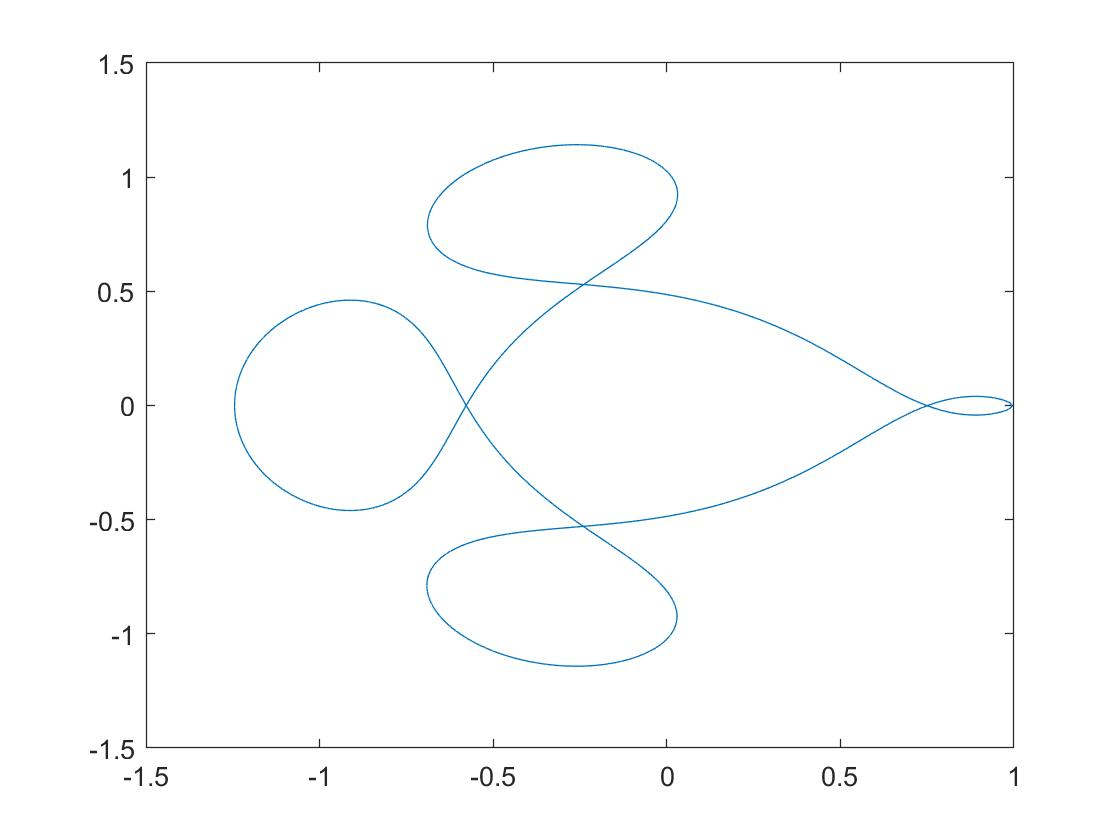
\includegraphics[height=0.35\textheight,width=0.7\linewidth]{1}
\caption{Result for actual case 1:Use Runge-Kutta method with 20000 steps.}
\end{figure}
\begin{figure}[H]
\centering
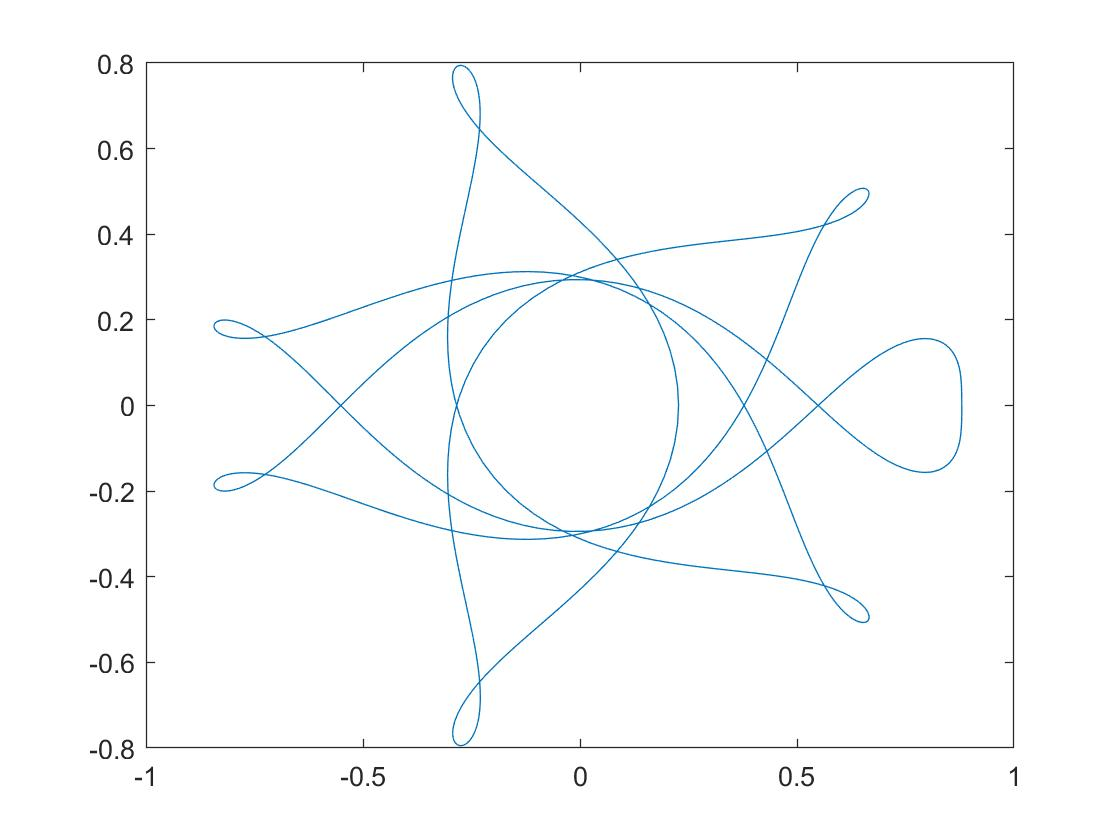
\includegraphics[height=0.35\textheight,width=0.7\linewidth]{2}
\caption{Result for actual case 2:Use Runge-Kutta method with 1000 steps.}
\end{figure}
\subsection{Straight-Forward Comparison}
\textbf{Remark:All the ODE-solver algorithms are based on equidistant partition!So I use the parameter "Step number" instead of "Time step".The relationship:$k=\frac{T}{n}$, $k$:time step,$n$:step number,$T$:the period.}

In this section,I make some comparison by straight-forward naked eye comparison.Rule:I will show the minimal stepnum to generate the figure similar to the correct ones.
\begin{table}[H]
\centering
\begin{tabular}{|l|l|l|}
\hline
Method                          & Precision & Stepnumber            \\ \hline
\multirow{4}{*}{Adam-Bashforce} & 1         & \textgreater{}1000000 \\ \cline{2-3} 
                                & 2         & near 250000           \\ \cline{2-3} 
                                & 3         & near 60000            \\ \cline{2-3} 
                                & 4         & near 50000            \\ \hline
\multirow{4}{*}{Adam-Moulton}   & 2         & near 125000           \\ \cline{2-3} 
                                & 3         & near 40000            \\ \cline{2-3} 
                                & 4         & near 25000            \\ \cline{2-3} 
                                & 5         & near 18000            \\ \hline
\multirow{4}{*}{BDF}            & 1         & \textgreater{}1000000 \\ \cline{2-3} 
                                & 2         & near 200000           \\ \cline{2-3} 
                                & 3         & near 40000            \\ \cline{2-3} 
                                & 4         & near 28000            \\ \hline
RungeKutta                      & 4         & near 18000            \\ \hline
\end{tabular}
\caption{The stepnum for actual case 1}
\end{table}
\begin{table}[H]
\centering
\begin{tabular}{|l|l|l|}
\hline
Method                          & Precision & Stepnumber            \\ \hline
\multirow{4}{*}{Adam-Bashforce} & 1         & \textgreater{}1000000 \\ \cline{2-3} 
                                & 2         & near 8000             \\ \cline{2-3} 
                                & 3         & near 6000             \\ \cline{2-3} 
                                & 4         & near 2000             \\ \hline
\multirow{4}{*}{Adam-Moulton}   & 2         & near 5000             \\ \cline{2-3} 
                                & 3         & near 3000             \\ \cline{2-3} 
                                & 4         & near 1500             \\ \cline{2-3} 
                                & 5         & near 1000             \\ \hline
\multirow{4}{*}{BDF}            & 1         & \textgreater{}1000000 \\ \cline{2-3} 
                                & 2         & near 5000             \\ \cline{2-3} 
                                & 3         & near 3500             \\ \cline{2-3} 
                                & 4         & near 1350             \\ \hline
RungeKutta                      & 4         & near 750              \\ \hline
\end{tabular}
\caption{The stepnum for actual case 2}
\end{table}
\section{Analysis:Precision and Relative Error}
\subsection{Analyze the Relative Error}
The definition of Relative Error comes as:
$$
E=\frac{||I_{E}-I_{A}||_{2}}{||I_{E}||_{2}}
$$
where $I_{E}$ denotes the actual solution,and $I_{A}$ denotes the solution approximated by the algorithm.Now, I will use actual problem (1) to do the test. 

Here is the result.Timestep N gets 100000.
\begin{table}[H]
\begin{tabular}{|l|l|l|l|l|}
\hline
Method                        & Precision & E(N)     & E(2N)    & E(4N)    \\ \hline
Adam-Bashforce                & 1         & 0.861674 & 0.829466 & 0.809348 \\ \hline
                              & 2         & 0.947447 & 0.784596 & 0.550436 \\ \hline
                              & 3         & 0.129373 & 0.012894 & 0.002843 \\ \hline
                              & 4         & 0.12506  & 0.019344 & 0.006423 \\ \hline
\multirow{4}{*}{Adam-Moulton} & 2         & 0.586927 & 0.322605 & 0.113165 \\ \cline{2-5} 
                              & 3         & 0.067277 & 0.029633 & 0.016107 \\ \cline{2-5} 
                              & 4         & 0.041897 & 0.026324 & 0.015617 \\ \cline{2-5} 
                              & 5         & 0.050341 & 0.026847 & 0.015557 \\ \hline
\multirow{4}{*}{BDF}          & 1         & 0.952406 & 0.966053 & 0.94306  \\ \cline{2-5} 
                              & 2         & 0.735703 & 0.579029 & 0.312331 \\ \cline{2-5} 
                              & 3         & 0.091682 & 0.031460 & 0.015582 \\ \cline{2-5} 
                              & 4         & 0.036067 & 0.014236 & 0.013965 \\ \hline
RungeKutta                    & 4         & 0.208489 & 0.010726 & 0.000697 \\ \hline
\end{tabular}
\end{table}
\subsection{Richardson Extrapolation Method}
Now, I will use \textbf{Richardson Extrapolation Method} to generate the convergent order.

In general problems, we can't get some information about the actual solution.So we need \textbf{Richardson extrapolation method.}For this problem, the equivalence comes as:
$$
p\approx log_{2}(\frac{||U(h)-U(\frac{h}{4})||_{2}}{||U(\frac{h}{2})-U(\frac{h}{4})||_{2}}-1)
$$
where $U(h)$ means the algorithm solution using time step h.The proof of this equation is shown in Levesque <Finite Differential Methods for Ordinary and Partial Differential Equations>, page 257.

In actual work,we can't set h too big or too small.If h is too big, the identity may not true, even the numerical form maybe unstable.If h is too small, it means we have to do something like "divide a small number", which is bad-conditioned.

Here are the results for the extrapolation method test:
% Please add the following required packages to your document preamble:
% \usepackage{multirow}
\begin{table}[H]
\centering
\begin{tabular}{|l|l|l|l|}
\hline
Method                          & Precision & Stepnumber(N) & test p      \\ \hline
\multirow{4}{*}{Adam-Bashforce} & 1         & 80000         & 0.70        \\ \cline{2-4} 
                                & 2         & 16000         & 1.72        \\ \cline{2-4} 
                                & 3         & 8000          & 2.92        \\ \cline{2-4} 
                                & 4         & 2000          & 3.69        \\ \hline
\multirow{4}{*}{Adam-Moulton}   & 2         & 1000          & 1.89        \\ \cline{2-4} 
                                & 3         & 850           & 2.79        \\ \cline{2-4} 
                                & 4         & 700           & 4.24        \\ \cline{2-4} 
                                & 5         & 180           & 5.21        \\ \hline
\multirow{4}{*}{BDF}            & 1         & 50000         & 2.28(a bug) \\ \cline{2-4} 
                                & 2         & 16000         & 1.78        \\ \cline{2-4} 
                                & 3         & 8000          & 2.71        \\ \cline{2-4} 
                                & 4         & 1500          & 4.68        \\ \hline
RungeKutta                      & 4         & 100           & 4.34        \\ \hline
\end{tabular}
\end{table}
\section{A contest:Forward Euler(1-order Adam-Bashforce) versus Classical Runge-Kutta}
Forward Euler algorithm and Classical Runge-Kutta algorithm are two famous algorithms in ODE solver.Now, I will compare these two algorithms in two means.
\subsection{Compare the result trajectory}
First of all,I will compare the 6000-steps result by RungeKutta with the 24000-steps result by ForwardEuler.I use actual case 1 to make a test.

Here are the results:
\begin{figure}[H]
\centering
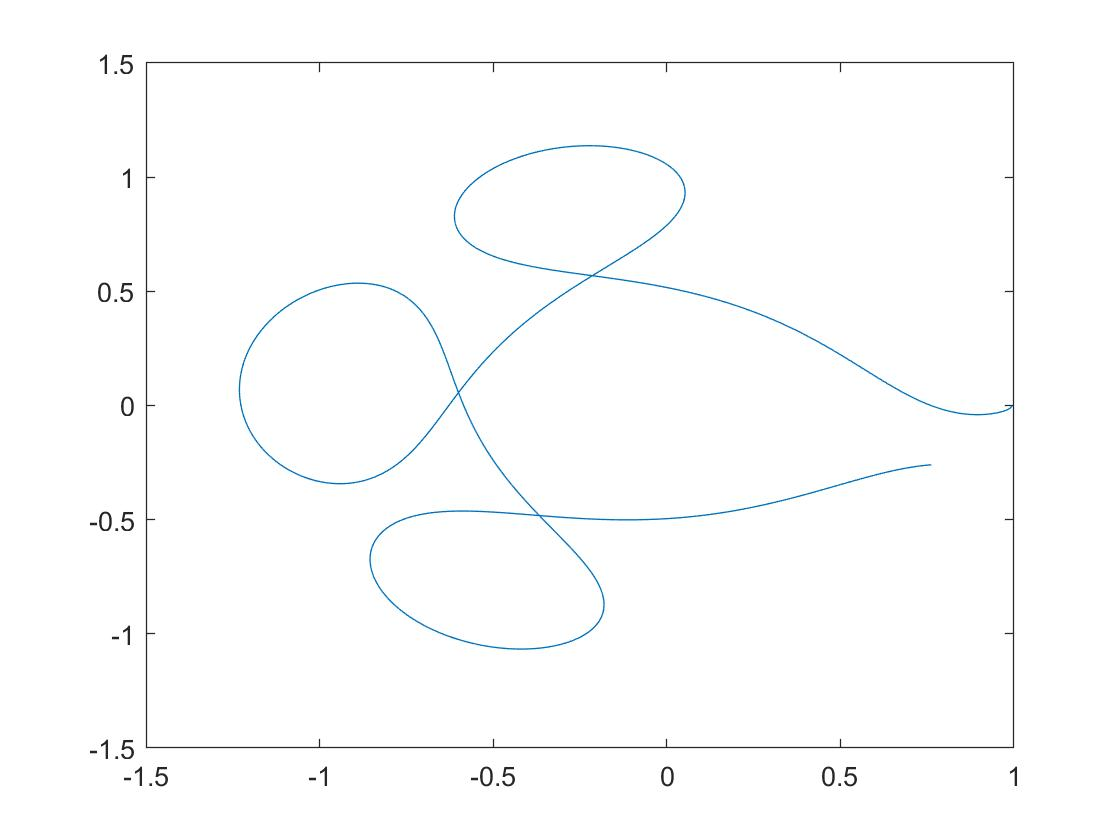
\includegraphics[height=0.35\textheight,width=0.7\linewidth]{3}
\caption{Result for actual case 1:Use Runge-Kutta method with 6000 steps.}
\end{figure}

\begin{figure}[H]
\centering
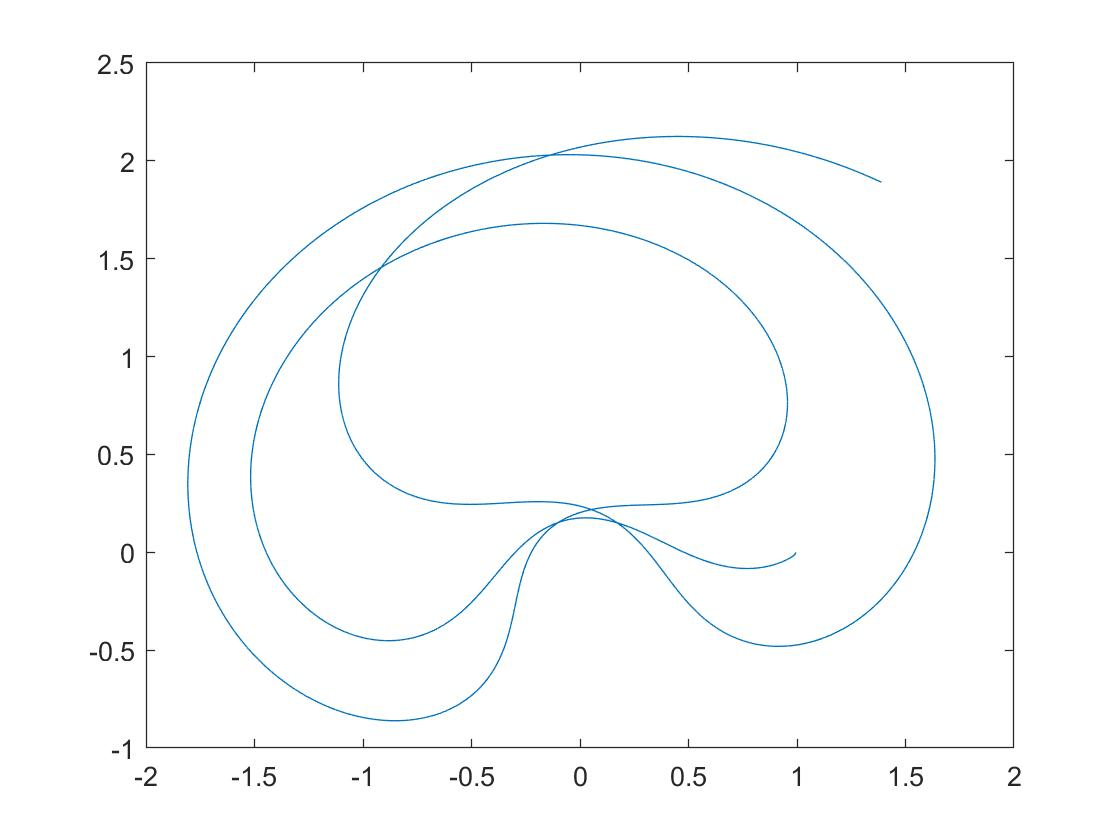
\includegraphics[height=0.35\textheight,width=0.7\linewidth]{4}
\caption{Result for actual case 1:Use Forward-Euler method with 24000 steps.}
\end{figure}

It's clear that:although the number of steps is different, Runge-Kutta algorithm performs far better than Forward-Euler algorithm.
\subsection{Compare the total CPU time}
Now, if we hope our result to achieve an error of $10^{-3}$ based on the maxnorm of the solution error, which algorithm will triamph?

\begin{figure}[H]
\centering
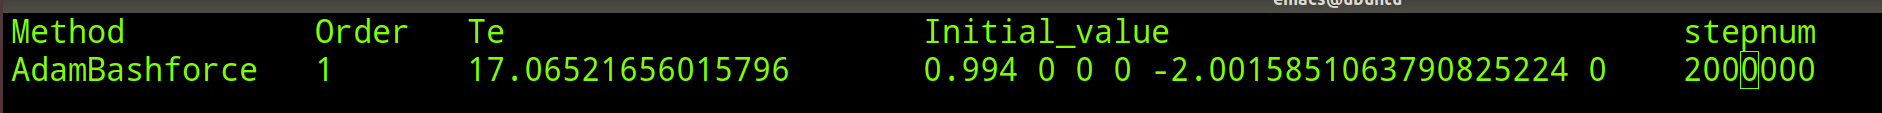
\includegraphics[height=0.05\textheight,width=0.9\linewidth]{5}
\caption{Input File for ForwardEuler}
\end{figure}
\begin{figure}[H]
\centering
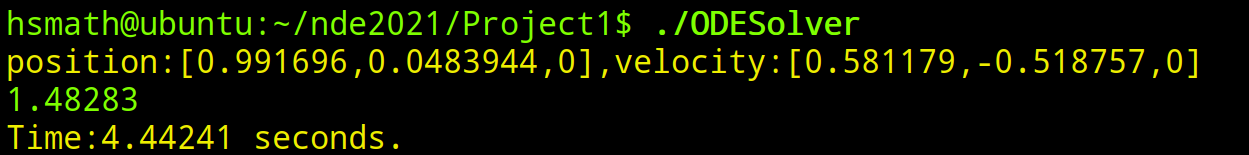
\includegraphics[height=0.1\textheight,width=0.9\linewidth]{6}
\caption{Result for the Forward Euler}
\end{figure}
What a pity!Although I set the step number to 2000000, the Forward Euler algorithm can't achieve my demand!The CPU time comes to 4.44241 seconds.

How about Runge-Kutta Method?
\begin{figure}[H]
\centering
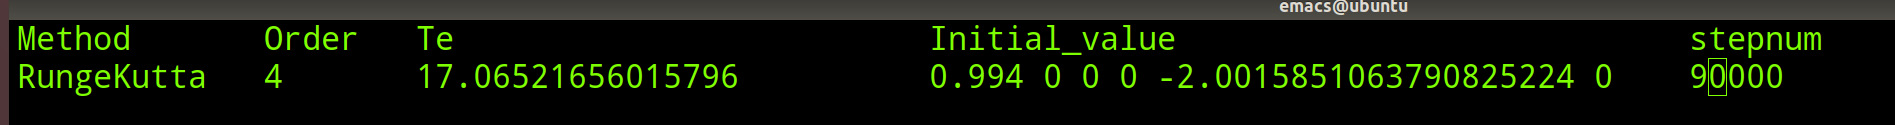
\includegraphics[height=0.05\textheight,width=0.9\linewidth]{7}
\caption{Input File for ForwardEuler}
\end{figure}
\begin{figure}[H]
\centering
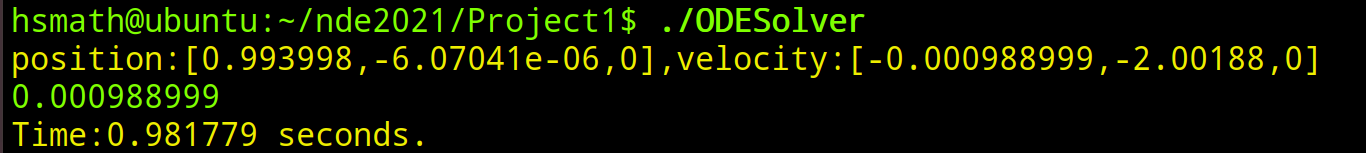
\includegraphics[height=0.1\textheight,width=0.9\linewidth]{8}
\caption{Input File for ForwardEuler}
\end{figure}

We can see:Runge-Kutta Method achieves my demand perfectly!And its CPU time is only 0.981779 seconds.

So, Runge-Kutta method must be the winner in this problem.

\section{Some shortcomings and doubts}
My package has the following shortcomings:
\begin{itemize}
\item Only use trivial time step.
\item The data structure isn't always same.In "Point" class, I use 3-dimension array to store the position and velocity, but when it comes to implicit difference scheme, I use Eigen::Matrix.
\item I didn't use template, which makes my program hard to reuse.
\end{itemize}

In additional, during the process of testing and coding, I have some doubts about this project.
\begin{itemize}
\item First-order algorithm usually convergent to a wrong answer,why?
\item The performance of Runge-Kutta method seems greater than LMM algorithms with precision = 4, why?
\item First of all, I try to generate the initial-value of LMM by Euler's Method, it happens that the precision of LMM reduce rapidly.What's more, the algorithm with precision = 2 performs better than p = 3, and better than p = 4.After I have done the Runge-Kutta algorithm, I try to generate the initial-value with RK algorithm, then everything goes right.What happens?
\end{itemize}
\section{Technical Details}
See the file "Readme.md"
\end{document}